\section{Results V: how black are the black boxes?}\label{sec:yardstick}

\subsection{Design}
For each teacher and series we fit, at the start of every calendar year $Y$, an SMoE shadow to ten
draws from the teacher's \emph{out-of-sample} predictive distribution on every earlier date, and use
the shadow to forecast year $Y$. The first three years of each teacher's out-of-sample history serve
as burn-in, so the shadow is evaluated from 2015 onwards on most series. The shadow never sees a
realised return: it learns only what the teacher predicted, and it learns it with information
available at the time. The reference model for the fidelity ratio is the historical Gaussian.
\Cref{tab:yardstick} summarises; \cref{fig:yardstick} shows every series.

\subsection{The deep SMoE is 92\% white}
The deep heterogeneous MoE improves on the historical Gaussian by a median of $0.129$ nats per day.
Its SMoE shadow achieves $0.122$, a median fidelity of $\Phi=0.92$ with interquartile range
$[0.89,0.96]$. The shadow reproduces the deep model's predictive variance almost exactly (median
$R^2$ of log variance $0.88$) but not its predictive mean ($R^2=0.20$), which is consistent with
\cref{sec:results-global}: the deep model's means carry no out-of-sample information, so there is
nothing for a white box to reproduce. The remaining eight percent is not noise: the
Amisano--Giacomini test rejects equal log scores of teacher and shadow on 12 of 19 series, always in
the teacher's favour. The black box knows a little more than three readable regimes do, and the
fidelity ratio measures how much more.

The probes give a complementary reading. The deep model's gate is \emph{not} a function of the
SMoE's state variables: linear probes of its gate logits on volatility, momentum and drawdown have
$R^2$ between $0.04$ and $0.84$ with a median of $0.26$, and only 9 of 57 expert-series probes exceed
$0.5$. The deep network therefore routes observations differently from the SMoE but ends up with
almost the same predictive distribution. When two different internal mechanisms produce the same
input--output map, inspecting internal weights (as the undergraduate thesis did with its gating
plots) can mislead, whereas a yardstick defined on the output cannot.


\subsection{Gradient boosting, Markov switching and GARCH}
The boosted model's shadow reproduces all of its gain ($\Phi=1.03$; log-variance $R^2=0.99$): its
predictive distribution is, to a first approximation, a log-HAR variance with a noisy mean. The
Markov-switching regression has $\Phi=0.93$ with the widest dispersion, reflecting that its latent
regime is filtered from past returns rather than from observables. GARCH-$t$ has $\Phi=0.98$, a useful
sanity check: the SMoE family contains close approximations to the GARCH predictive.

\subsection{Foundation models: the shadow beats the teacher}
The zero-shot Chronos-Bolt forecasts are no better than the historical Gaussian on the median
series (gain $-0.054$ for the small and $-0.004$ for the base model), because their predictive
distributions are too narrow (PIT standard deviations $1.32$ and $1.25$; \cref{sec:results-global}).
Their SMoE shadows, fitted to the same forecasts, gain $+0.035$ and $+0.062$. The small model's shadow
beats its teacher on every series, significantly on 15 of 19; the base model's shadow beats its
teacher on 17 series, significantly on 14. Scaling the foundation model improves its calibration, but
not enough to close the gap to its own white-box reading.

TimesFM~2.5, a different architecture released ten months after Chronos-Bolt, is the first foundation model in
our comparison that beats the historical Gaussian on the median series, by $0.012$ nats per day; its
PIT standard deviation of $1.17$ is the closest to one among the three. The pattern is nevertheless
the same. Its shadow gains $0.043$, beats its teacher on 14 of 19 series and does so significantly on
10, while the teacher is never significantly better than its shadow. Projecting a foundation model
onto a structured likelihood family therefore acts as a regulariser: the shadow keeps the information
in the teacher's location and relative-scale forecasts (median log-variance $R^2$ between $0.48$ and
$0.57$ for the three models) while the semantic variance experts re-anchor the overall scale to the
data. For the Chronos models fidelity is negative because the teacher loses to the reference, and for
TimesFM the teacher's gain is too small for the ratio $\Phi=0.46$ to be read as a share. The common
finding is that none of the three foundation models produces a predictive distribution that is
usable as is, while a white-box reading of each one is.


\begin{figure}[t]\centering
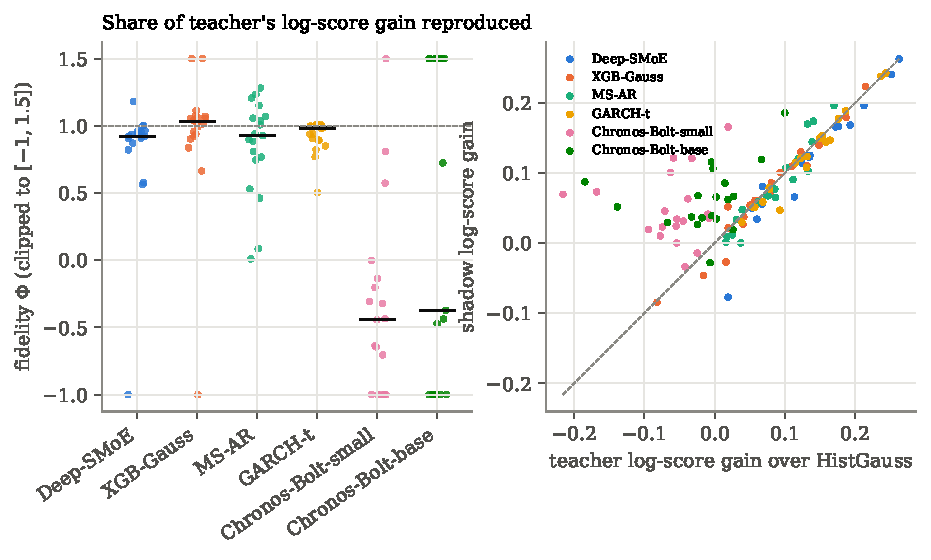
\includegraphics[width=\textwidth]{../results/figures/yardstick.pdf}
\caption{The white-box yardstick. Left: fidelity $\Phi$ per teacher and series (horizontal bars are
medians). Right: out-of-sample log-score gain over the historical Gaussian of each teacher ($x$)
and of its SMoE shadow ($y$); points above the diagonal are series on which the shadow beats its
teacher.}\label{fig:yardstick}
\end{figure}

\begin{table}[!htbp]\centering\scriptsize
\caption{The white-box yardstick: fidelity of SMoE shadows of black-box forecasters (out of sample)}\label{tab:yardstick}
\begin{adjustbox}{max width=\textwidth}
\begin{tabular}{lrrrrrrrr}
\toprule
Teacher & Series & Median LS gain & Median $\Phi$ & $R^2$ mean & $R^2$ log var & $R^2$ P(up) & Median KL & AG reject\\
\midrule
Chronos-Bolt-base & 19 & -0.004 & -0.373 & 0.109 & 0.566 & 0.157 & 0.052 & 14\\
Chronos-Bolt-small & 19 & -0.054 & -0.443 & 0.143 & 0.478 & 0.244 & 0.063 & 15\\
Deep-SMoE & 19 & 0.129 & 0.922 & 0.198 & 0.877 & 0.175 & 0.019 & 12\\
GARCH-t & 19 & 0.131 & 0.983 & 0.003 & 0.804 & 0.249 & 0.016 & 5\\
MS-AR & 19 & 0.086 & 0.927 & 0.282 & 0.579 & 0.379 & 0.025 & 9\\
XGB-Gauss & 19 & 0.060 & 1.032 & 0.013 & 0.986 & 0.035 & 0.007 & 5\\
\bottomrule
\end{tabular}
\end{adjustbox}
\par\smallskip\begin{minipage}{\textwidth}\footnotesize
LS gain: teacher log score minus historical-Gaussian log score. $\Phi$: share of that gain reproduced by the SMoE shadow. AG reject: number of series on which the Amisano--Giacomini test rejects equal log scores of teacher and shadow at 5\%.
\end{minipage}
\end{table}
